%%%%%%%%%%%%%%%%%%%% author.tex %%%%%%%%%%%%%%%%%%%%%%%%%%%%%%%%%%%
%
%%%%%%%%%%%%%%%% Springer %%%%%%%%%%%%%%%%%%%%%%%%%%%%%%%%%%

\newfloat{Query}{tbp}{lop}

\title*{Using Graph Databases to Explore Genetic Programming Run Dynamics}
% Use \titlerunning{Short Title} for an abbreviated version of
% your contribution title if the original one is too long
\author{Nicholas Freitag McPhee, David Donatucci, and Thomas Helmuth and others(?)}
% Use \authorrunning{Short Title} for an abbreviated version of
% your contribution title if the original one is too long
\institute{Nicholas Freitag McPhee \at University of Minnesota, Morris
\and David Donatucci \at University of Minnesota, Morris
\and Thomas Helmuth \at University of Massachusetts Amherst}

\maketitle

\abstract{Each chapter should be preceded by an abstract (10--15 lines long) that summarizes the content. The abstract will appear \textit{online} at \url{www.SpringerLink.com} and be available with unrestricted access. This allows unregistered users to read the abstract as a teaser for the complete chapter. As a general rule the abstracts will not appear in the printed version of your book unless it is the style of your particular book or that of the series to which your book belongs.}

\begin{keywords}
keywords to your chapter, these words should also be indexed
\end{keywords}
\index{keywords to your chapter}
\index{these words should also be indexed}
\\

\section{Introduction}
\label{sec:introduction}

It is common practice in most empirical evolutionary computation (EC) 
research\marginpar{It would be nice to scrape, say, the GECCO 2014 proceedings and get some 
	numbers to back this up.} to perform numerous (possibly hundreds) of runs, and then simply 
report a handful of aggregate statistics at the end that are expected to summarize and represent 
the (hopefully) complex interactions and dynamics of those many runs. Tables present values such 
as mean or median best fitnesses at the end of runs, collapsing the complexities of dozens or 
hundreds of runs into a single number, possibly with a standard deviation or (even better) a 
confidence interval to give a sense of the distribution. Often more informative are plots, which can, 
for example, show how these numbers change over time during the runs, possibly giving a sense of 
the system dynamics. These plots, however, often aggregate runs in a way that obscure important 
moments that, if explored, might reveal valuable insight into the evolutionary dynamics being 
reported.

An alternative would be to collect, store, and analyze at least some of the rich panoply of 
evolutionary and genealogical events that make up the vital low-details details of these runs. 
Databases provide a natural tool for 
storing and accessing the data, but traditional relational
databases are poorly suited for a variety of queries that are important for the genealogical analysis
we need for exploring the evolutionary dynamics of our EC runs. \marginpar{Removed this bit since we talk about it in the neo4j subsection now. Is this a good combination of paragraphs?} %If, for example, we have a 
%\texttt{ParentChild} table, it's easy enough to find Alice's parents. Finding Alice's grandparents,
%siblings, or cousins, however, is less straightforward, with queries becomes increasingly difficult
%as we move farther out across the relationship tree.
In this chapter, we illustrate the use of graph databases as an alternative storage and analysis tool for
evolutionary computation runs. In \cite{donatuccianalysis} we have demonstrated that graph databases
can be an effective tool for analyzing complex genetic programming (GP) dynamics, which led directly
to a proposed change to standard sub-tree crossover in tree-based GP, \cite{mcphee:GECCO15}.
Here we will use the open source Neo4J graph database tool\footnote{\url{http://neo4j.com/}} 
to explore data from a
collection of PushGP runs on several problems drawn from a benchmark collection of introductory 
programming problems taken from \cite{helmuth:GECCO15}.

Note that this is \emph{not} going to be a presentation of ``traditional'' ``hypothesis-driven'' 
research. It will be based on an \emph{assumption}, namely that something interesting happens in
these runs, and that we can learn useful things by exploring them in more detail, but the presentation
will be fairly discursive, reflecting our back-and-forth experience of wrestling with the data. Our
initial queries start from fairly obvious questions (e.g., ``Why did we succeed here?''), but from
there we have a dialog with data, letting the answers to early questions shape and guide our 
subsequent exploration. We are presenting not the tidy, sterile summary of our adventures, but
the messier (but we think more informative in this context) journal of what Pickering would call
our ``mangle of practice'' (\cite{smith2008mangle, pickering:AJS:1993}).

\emph{More stuff would have to be added here, including a roadmap.}

\section{Motivation}
\label{sec:motivation}

Consider the job of a paleontologist, who regularly reconstructs not just individuals but also
species and entire phylogenetic trees on the basis of handful of teeth and bones, or even just
impressions left in prehistoric mud. They rarely have DNA, so any evolutionary relationship is
inherently speculative, subject to constant debate and revision. Even with detailed DNA sequences,
the construction of phylogenetic trees for existing species is a challenge.\marginpar{A reference
	for all of this phylogenetic reconstruction stuff would be useful.}

In evolutionary computation, however, we have access to \emph{everything}, at least in principle. Every
selection, every mating, every mutation, and every crossover happens in our code and on our watch.
Yet we typically throw almost all that data away, reporting just aggregate statistics and summary
plots, completely failing to take advantage of our privileged position, a position most 
paleontologists would presumably eye with considerable envy. Not only does this seem an inherent
waste, these aggregations typically obscure critical moments in the dynamics of runs which might
speak volumes if explored.
\marginpar{Perhaps include a sample plot and show how it hides things? One of Tom's 
	diversity or cluster plots? A synthetic plot? Maybe that's just not necessary?}

While this sort of aggregate reporting is often valuable, allowing for important comparative
analysis of, for example, the impact of different genetic operators, it typically fails to provide
any sense of the \emph{why}. Yes, Treatment A led to better aggregate performance than 
Treatment B -- but what happened in the runs that led to that result? Any success at the end of a
run is ultimately the intricate combination of hundreds or thousands of selections, recombinations
and mutations, and if Treatment A is in some sense ``better'' than Treatment B, it must ultimately
be because it affected all those genealogical and genetic events in some significant way, biasing them
towards events that made success more likely.

Unfortunately, published research very rarely includes information that might shed light on 
these \emph{why} events. We rarely see evolved programs, for example, or any kind of post-run analysis
of those programs, and there is almost never any data or discussion of the genealogical history that
might help us understand how a successful program actually came to be. 
Sometimes these events and details aren't included
for reasons of space and time; evolved programs, for example, are often extremely large and complex,
and a meaningful presentation and discussion of such a program could easily take up more space than
authors have available given the typical space limitations in published work.
Our suspicion, however, is that another reason this sort of \emph{why} analysis often isn't 
reported is because it isn't done, in no small part because it's hard. As EC researchers we're in the
``privileged'' position of being able to collect anything and everything that happens in a run, 
but that's a potentially huge amount of data, and leaves us with two substantial problems: 
How to \emph{store} the data, and how to \emph{analyze} the data
after it's stored. 

%Decreasing data storage costs have done much to mitigate the first problem.
%If, however, one collects a very rich data set it's still easy to quickly generate terabytes of data,
%and even if one has a place to put the data, one still needs reasonable tools to analyze the data.

Assuming one has access to the necessary gigabytes or terabytes of storage, 
databases are the obvious tool for the collection of the data. Most common database structures and tools,
however,
don't lend themselves to the kinds of analysis that we want and need in evolutionary computation work. Most relational and document-based databases, for example require things like complex and expensive 
recursive joins to trace significant hereditary lines, making this approach increasingly unfeasible.
 In exploring the dynamics of an EC run, we're going to want to be able to
make connections across dozens or even hundreds of generations, which simply isn't plausible with a
relational database. (See~\cite{Robinson:GraphDB:Book} for more on these 
feasability/efficiency issues.) While we decided to utilize Neo4j as our graph database, there are other graph databases that would be an effective tool to use as well see~\cite{wiki:GraphDB}. 

\emph{Say a little about how graph databases rock on this and that's why we're using them here. Also
	mention that Neo4J isn't the only option out there; it just happens to be the one that we're
	using.}

\section{A little background on problems and tools}

\subsection{Neo4J and Cypher}
\label{subsec:Neo4j}
Graph databases~%\cite{GraphDatabases:2013}
 are a relatively new approach, where data is stored as a collection of nodes and relationships in a graph, with a specialized query language that makes it easy to ask questions about complex relationships. This section further describes Neo4j, its query language Cypher, and the various advantages they hold over relational databases in recording and accessing information that relies heavily on recursion.

Neo4j is a form of data management system based upon a graph. Information is stored by means of vertices and edges, commonly referred to as nodes and relationships, respectively~%\cite{GraphDatabases:2013}
. In our work, nodes represent individuals, and relationships represent the transformations between individuals. As a GP system generates individuals, new nodes and relationships can be added to the database for later analysis.

Cypher%~\cite{GraphDatabases:2013}
 allows this data to be readily extracted from the Neo4j database. There are three fundamental elements to queries in Cypher. The \texttt{START} clause specifies a starting location in the database, indicating the node or nodes where the query will begin. The \texttt{RETURN} clause specifies which nodes, relationships, or properties should be returned to the user. The \texttt{MATCH} clause is the main section of a query, specifying what patterns in the graph the query will discover. To write the \texttt{MATCH} clause, nodes and relationships are drawn with ASCII characters. A node is indicated by parenthesis \texttt{( )}, directed relationships are indicated with \texttt{-->} or \texttt{<--} depending on the direction of the relationship, and undirected relationships are indicated with \texttt{--}. Brackets \texttt{[ ]} between the dashes can be used to specify relationship names prefixed by a colon. In the example query below, the \texttt{START} clause indicates that the query should start with node 43, called \texttt{parent}, the \texttt{MATCH} clause finds all nodes that are children of the starting node, and the \texttt{RETURN} clause yields the starting node and all nodes that are children of that node.

\begin{verbatim}
    START parent=node(43)
    MATCH (parent)-[:PARENTOF]->(child)
    RETURN parent, child;
\end{verbatim}

%This query produces the results in Figure \ref{fig:exampleQuery}.
\begin{figure}[tb]
 \sidecaption[t]
 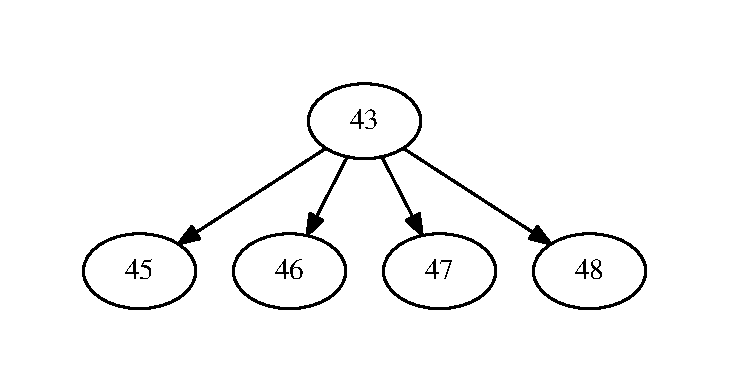
\includegraphics[width=0.8\textwidth]{figures/sample_neo4j_query.pdf}
 \caption{Graphical representation of the results of a sample Cypher query}
 \label{fig:exampleQuery}
\end{figure}

Performance is the key advantage in our research of graph databases over relational databases. As the data set grows, recursive queries such as those needed to explore graph relationships become highly inefficient when using relational databases, as numerous joins are needed. In graph databases, however, the portion of the data set that must be searched is limited because the query will only search along an available path connected by relationships, allowing queries to remain efficient~%\cite{GraphDatabases:2013}.


\subsection{PushGP and lexicase selection}

Say a little about
\begin{itemize}
	\item Plush genomes
	\item Push programs
	\item Alternation
	\item The two kinds of mutation
\end{itemize}

Say enough about lexicase so people have some sense of why it might be interesting and different
from, e.g., tournament selection.

Mention timing out and errors penalties.

\subsection{Replace-space-with-newline}

Say enough about this problem so that people can understand the error vectors.

\section{Lexicase, meet Replace-space-with-newline}
\label{meetLexicase}
We did one hundred runs of the replace-space-with-newline problem using lexicase selection, and
found that 55 of these succeeded in the sense that an individual was discovered that had zero
error on all 200 of the training cases. Tournament selection with tournament size 7 only
had 13 successes out of 100 runs, and IFS only had 17 successes out of 100 runs, so it seems that
lexicase selection provides a significant advantage here.

\subsection{Hey, we won! But how did we get there?}

% This is run 6, lexicase, replace-space-with-newline.

Interestingly enough, lexicase performed very well, but this leaves us with the crucial question of \emph{why}? 
In order to answer this question, we chose one successful run to explore in more detail. However, it's important to note
here that we're making no claims that this is a ``representative'' run (whatever that would even
mean); it's an \emph{interesting} run, though, and our hope is that by understanding its dynamics
better we can learn useful things about both the problem and the tools we're applying.

\begin{sidewaysfigure}
	\vspace{0.6\columnwidth}
	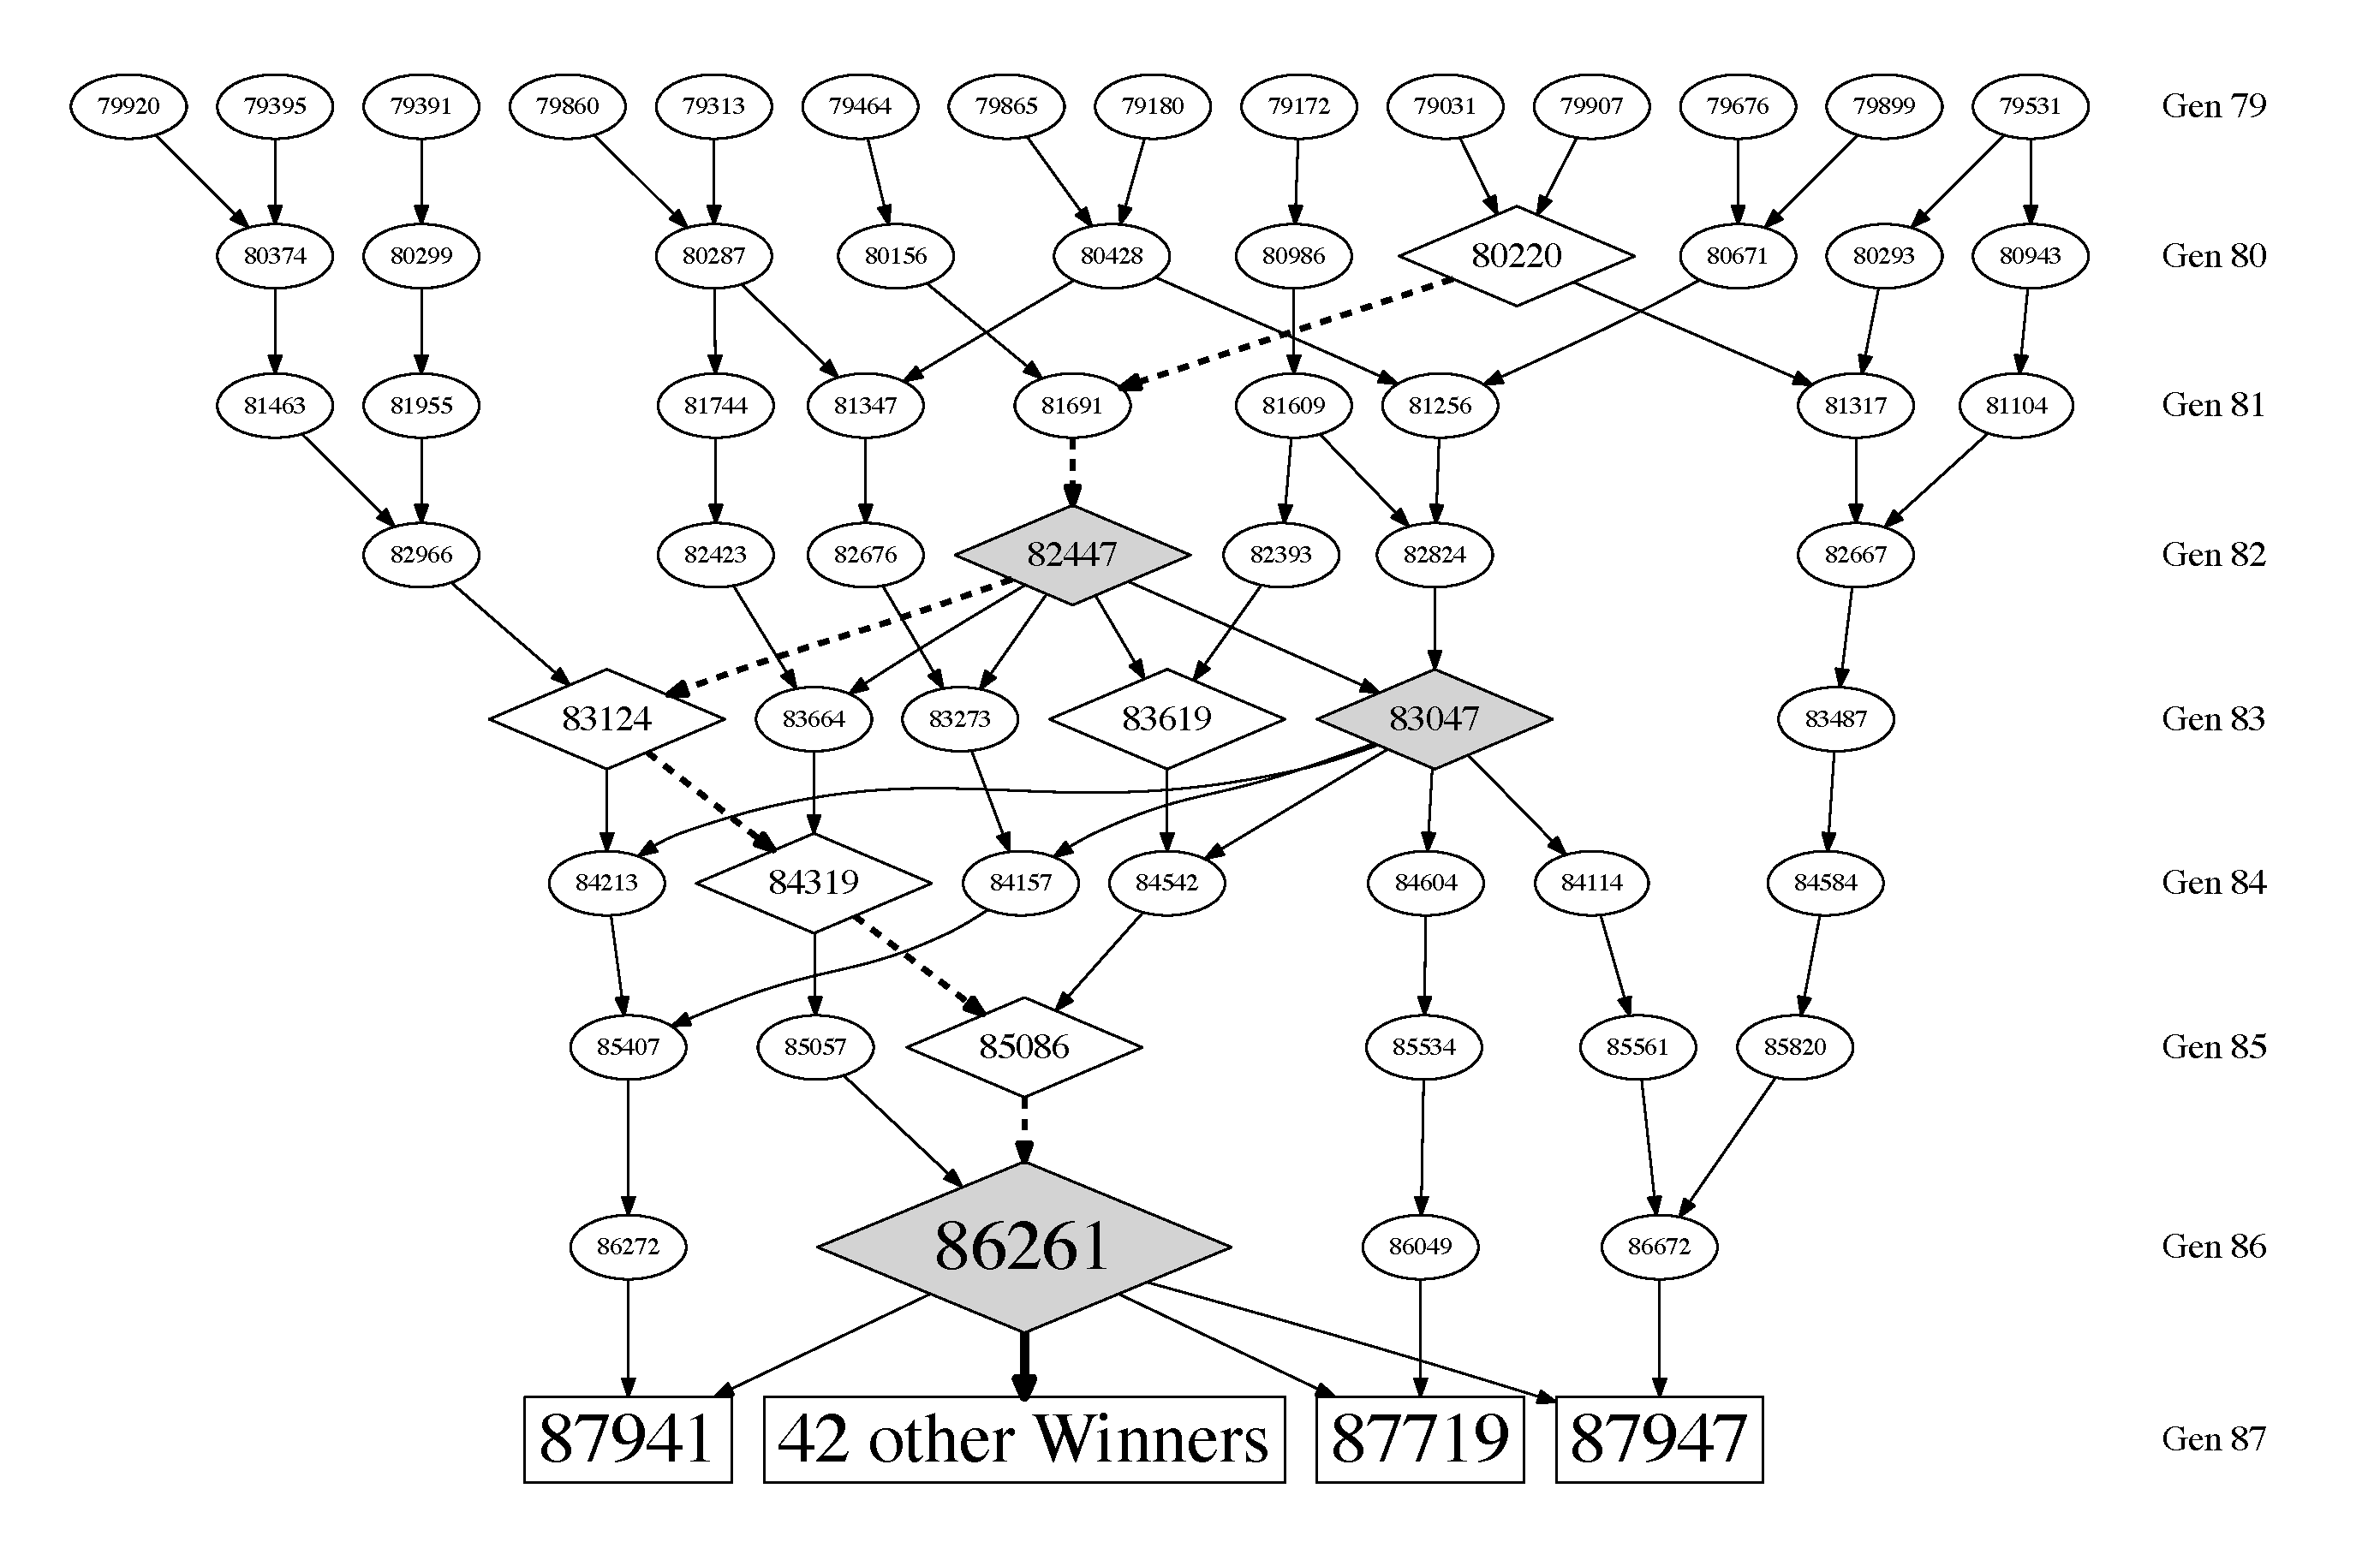
\includegraphics[width=0.88\columnwidth]{figures/ancestors_of_winners.pdf}
	\caption{Ancestry of the 45 ``winners'' from run 6 of lexicase, replace-space-with-newline. Nodes
		with diamonds instead of ellipses had an unusually large number of offspring. Shaded nodes
		had an unusual number of offspring that were ancestors of winners. The dashed lines highlight
		individuals that had an unusually large number of distinct ancestry paths down to a winner.
		See the text for more details}
	\label{fig:winnerAncestors}
\end{sidewaysfigure}

An obvious place to start analyzing is at the end when the GP system created individuals that solved the problem. So we used Neo4J to find all the ancestors of any ``winning'' individual, i.e., individual with a total error of 
on all 200 test cases. Using Cypher%(Neo4J's query language)
, we can easily ask for this subset
of the population going back to generation 79 using the query in 
Query~\ref{query:winnerAncestors}.\footnote{We could certainly 
	have gone back farther in time, but the graph would have become impossible to read as the
	number of nodes would have ballooned from a few dozen to hundreds or thousands. We went
	back to generation 79 because that was the most recent generation that had more than 10
	distinct ancestors of a winning individual.}\marginpar{Should all the query details go in
	an appendix that eventually becomes a tech report or some such? I'm not sure if they aren't
	just a distraction here.}\marginpar{We need the crazy \texttt{p->c->w} thing in 
	Query~\ref{query:numChildren} to extract 
	single edges, but I don't know if we want to talk about that.}

\begin{Query}
	\begin{verbatim}
	MATCH (p)-->(c)-[*0..7]->(w {total_error: 0}) 
	RETURN DISTINCT id(p), id(c);
	\end{verbatim}
	\caption{Cypher query to find all the ancestors of ``winners'' in the last 9 generations of a run.
		The pattern \texttt{(w \{total\_error: 0\})} matches nodes with total error 0, i.e., 
		``winners''. The pattern \texttt{(c)-[*0..7]->(w)} matches any path from some node \texttt{c} to
		a winning node \texttt{w} that has between 0 and 7 edges.
		}
	\label{query:winnerAncestors}
\end{Query}

Figure~\ref{fig:winnerAncestors} shows the ancestry of all of the winners from generation 87 
(when we first found a winner in this run) back to generation 79.
Each node in the graph represents an individual, and each directed edge indicates a parent-child
relationship, with the edge going from the parent to the child. The numbers inside the nodes are
Neo4J internal IDs; we'll use these as ``names'' for the individuals as we tell the stories we uncover.
\footnote{We actually assign each individual a UUID so we can combine multiple runs, but
	the Neo4J IDs are shorter and easier to use in our story telling.} As a happy accident coming
from having a population size of 1,000, the first two digits of the Neo4J idea also happens to indicate
what generation that individual was from.

Ignoring for the moment the adornments (shape, shading, etc.), there are several things that
we can observe right away:
\begin{itemize}
	\item There are 45 distinct winners in the final generation, or 4.5\% of the population of
	1,000 individual. This tells us that constructing a winner from the individuals in generation 86
	wasn't entirely trivial, but it also wasn't a huge challenge and happened multiple times.
	\item The 45 winners only had four distinct ancestors in the preceding generation.
	\item All 45 winners had a single individual (86261, marked with a large shaded diamond near
	the center bottom) as at least one of their parents, and 42 of
	them had 86261 as their \emph{only} parent, i.e., they were mutations of 86261, or were the result
	of self-crosses of 86261. To simplify the graph, we've combined those 42 individuals into a
	single node labeled ``42 other Winners''.
	\item The number of ancestors of winners doesn't grow quickly as we move back in time. We have to
	go back to generation 80 to find 10 individuals (or 1\% of the population) that are ancestors of
	winners, and in generation 79 there are still only 14 ancestors of winners. In fact, we have to
	go trace the ancestry all the way to generation 63 to find a time where over 100 individuals (or over 10\% of 
	the population) were ancestors of a winning individual.
\end{itemize}

\subsection{Surprising fecundity (especially given that total error)}
\label{sec:surprisingFecundity}

Looking at Figure~\ref{fig:winnerAncestors} we can see that a few individuals have more offspring
represented than others. As we've already mentioned, individual 86261 has 45 successful offspring,
and both individuals 82447 and 83047 have five offspring in the graph, i.e., five offspring that were
ancestors of a winning individual in generation 87. Each of these is marked in 
Figure~\ref{fig:winnerAncestors} with a shaded diamond.

Figure~\ref{fig:winnerAncestors},
however, only tells us how many offspring an individual had that were themselves either a winner
or an ancestor of a winner, as no other nodes are displayed. One
might, however, wonder how many total offspring an individual has
regardless of whether they were a winner or not. Query~\ref{query:numChildren} identifies the most
fecund ancestors of winners in these last nine generations. That reveals several results that were
quite surprising to at least some of the authors, the most remarkable being that individual 86261 
was a parent of 934 of the 1,000 individuals in generation 87! Given that lexicase selection was
designed in significant part of spread selection events out across the population, this makes it
clear that there are times when lexicase does the opposite, and instead puts nearly all its eggs in
a single basket. This level of selection focus would simply be impossible using almost any other
common type of selection such as tournament selection; in most uses of tournament selection, 
for example, no individual can be in more than a relative handful of tournaments, and thus can't be
a parent terribly often no matter how fit they are.

\begin{Query}
	\begin{verbatim}
	MATCH (p)-->(c)-[*0..7]->(w {total_error: 0}) 
	MATCH (p)-->(n) 
	RETURN DISTINCT id(p), count(DISTINCT n) 
	ORDER BY count(distinct n) DESC
	LIMIT 20;
	\end{verbatim}
	\caption{Cypher query to find, for each ancestor \texttt{p} of a winner, how many distinct offspring 
		\texttt{n} that ancestor \texttt{p}, regardless of whether \texttt{n} is itself an
		ancestor of a winner. The query then sorts by that count, and returns the 20 highest results.}
	\label{query:numChildren}
\end{Query}

% Go through ancestors of winners for last 9 generations, counting number of offspring, and returning
% the ``big'' winners.
%neo4j-sh (?)$ match (p)-->(c)-[*0..7]->(w {total_error: "0"}) match (p)-->(n) return distinct id(p), count(distinct n) order by count(distinct n) desc limit 20;
%+---------------------------+
%| id(p) | count(distinct n) |
%+---------------------------+
%| 86261 | 934               |
%| 82447 | 433               |
%| 84319 | 279               |
%| 80220 | 200               |
%| 85086 | 180               |
%| 83124 | 170               |
%| 83619 | 143               |
%| 83047 | 110               |
%| 79031 | 63                |
%| 80287 | 50                |
%| 79531 | 38                |
%| 79391 | 34                |
%| 79313 | 24                |
%| 82667 | 21                |
%| 82423 | 20                |
%| 83664 | 18                |
%| 80428 | 18                |
%| 81691 | 17                |
%| 80943 | 17                |
%| 80671 | 14                |
%+---------------------------+
%20 rows
%162649 ms

While no other node in Figure~\ref{fig:winnerAncestors} has nearly as many children as 86261 did,
there are several that also had very high reproduction rates, putting them well above what would be 
possible with something like tournament selection. Individual 82447, for example, had
443 offspring, including the 5 illustrated in Figure~\ref{fig:winnerAncestors}. In fact there were
eight individuals in Figure~\ref{fig:winnerAncestors} that have more than 100 offspring; each of
these is indicated with a diamond shape instead of the standard ellipse. This highlights a particularly
interesting ancestry chain from 80220 through 81691, 82447, 83124, 84319, 85086 to 86261, marked with
dashed edges in Figure~\ref{fig:winnerAncestors}. With the exception of 81691, which ``only'' had 17
offspring, each of these seven individuals had more
than 100 offspring, and thus had a fairly dominate role in shaping the generation that followed them. 

If we look at the total error in of the individuals in Figure~\ref{fig:winnerAncestors}, we again
find some significant surprises that tell us quite a lot about lexicase selection. In particular, if
we look at the total error for each individual along the dashed path from 80220 through
82447 to 86261, the fitness of the first five
individuals in the chain aren't too surprising. One (individual 82447) has the best total error in
that generation and all but 81691 (the individual with only 17 offspring) are in the top fifth of the 
population when ranked by total fitness. The fitnesses 
of the last two (the grandparent and parent of \emph{every} one of the 45 solutions), however, 
came as quite a shock. In particular, individual 85086 has a total error of 100,000, placing it
\emph{very near the bottom of the population by total error} (rank 971). Individual 86261, which was
the parent of 924 of the 1,000 individuals in the next generation, has a total error of 4,034, placing
it below $3/4$ of the population in its generation by that aggregate measure.

\begin{table}[t]
	%\sidecaption[t]
	\caption{The total error and rank (by total error) in the population in that individual's generation
		for the sequence of ``diamond'' individuals from in Figure~\ref{fig:winnerAncestors}.}
	\label{table:winnerFitnesses}
	\begin{center}
	\begin{tabular}{rrr}
		Individual & $\quad$ Total error & $\quad$ Rank in population \\
		\hline
		80220 & 321 & 147 \\
		81691 & 441 & 268 \\
		82447 & 107 & 1 \\
		83124 & 157 & 85 \\
		84319 & 240 & 188 \\
		85086 & 100,000 & 971 \\
		86261 & 4,034 & 765
	\end{tabular}
	\end{center}
\end{table}

So how could individuals with such terrible total fitness end up being selected so often as parents?
Exploring the specific test case errors reveals that individual 85086 is perfect on half of the test
cases (all those that involve printing), but gets a penalty error of 1,000 on the other half, presumably
because it never actually returns a value. Every one of its ancestors in 
Table~\ref{table:winnerFitnesses}, however, has at least a few non-zero errors on the printing
test cases, meaning that any lexicase ordering that places a few key printing test cases before
any of the ``return'' test cases would likely select individual 85086.

What about individual 86261, with it's 934 offspring? It is perfect (has error zero) on 194 of the 200
test cases, with it's total error of 4,034 coming from the remaining 6 test cases. On four of these it,
like individual 85086, fails to return a value and gets the penalty of 1,000; it has an error of 17 on
the other two. Thus it gets 97\% of the test cases correct, but happens to be \emph{heavily} penalized
for its behavior on 4 of the 6 it gets wrong. In a system that aggregates the errors, its rank of 765
out of 1,000 would mean that it would probably have no offspring. With lexicase selection, however,
it's success on the 194 test cases means that it is selected (from this population) almost every time.
In fact only 152 of the 1,000 individuals in the final generation had a parent who \emph{wasn't}
86261, and only 116 other individuals in generation 86 had an offspring in the next generation. While
four of those had 10 or more offspring in the last generation, none of those four actually
gave rise to a winner. The three parents of winners other than 86261 (individuals 86272, 86049, 
and 86672 in Figure~\ref{fig:winnerAncestors}) had very few offspring (1, 2, and 2 respectively),
suggesting that they may not have contributed much (or anything) to their successful progeny, and 
the success of their offspring was due more to the good fortune of mating with 86261 than anything else.

%neo4j-sh (?)$ match (n)-[* 1]->(m {generation: "87"}) return id(n), count(distinct m) order by count(distinct m) desc limit 40;
%+---------------------------+
%| id(n) | count(distinct m) |
%+---------------------------+
%| 86261 | 934               |
%| 86507 | 27                |
%| 86166 | 16                |
%| 86793 | 12                |
%| 86487 | 10                |
%| 86320 | 6                 |
%| 86608 | 6                 |
%| 86605 | 6                 |
%| 86434 | 4                 |
%| 86657 | 4                 |
%| 86211 | 4                 |
%| 86778 | 3                 |
%| 86736 | 3                 |
%| 86499 | 3                 |
%| 86356 | 3                 |
%| 86136 | 3                 |
%| 86562 | 3                 |
%| 86329 | 3                 |
%| 86516 | 3                 |
%| 86873 | 3                 |
%| 86150 | 2                 |
%| 86132 | 2                 |
%| 86213 | 2                 |
%| 86626 | 2                 |
%| 86052 | 2                 |
%| 86850 | 2                 |
%| 86949 | 2                 |
%| 86713 | 2                 |
%| 86130 | 2                 |
%| 86049 | 2                 |
%| 86775 | 2                 |
%| 86495 | 2                 |
%| 86475 | 2                 |
%| 86241 | 2                 |
%| 86815 | 2                 |
%| 86770 | 2                 |
%| 86975 | 2                 |
%| 86257 | 2                 |
%| 86933 | 2                 |
%| 86756 | 2                 |
%+---------------------------+
%40 rows
%766 ms
% tourneyment run 74 less selection pressure on one parent
%neo4j-sh (?)$ match (n)-[* 1]->(m {generation: 150}) return id(n), count(distinct m) order by count(distinct m) desc limit 40;
%+----------------------------+
%| id(n)  | count(distinct m) |
%+----------------------------+
%| 149373 | 17                |
%| 149998 | 15                |
%| 149701 | 15                |
%| 149050 | 14                |
%| 149885 | 13                |
%| 149822 | 13                |
%| 149985 | 13                |
%| 149447 | 13                |
%| 149920 | 13                |
%| 149711 | 13                |
%| 149091 | 13                |
%| 149063 | 12                |
%| 149418 | 12                |
%| 149164 | 12                |
%| 149577 | 12                |
%| 149414 | 12                |
%| 149037 | 12                |
%| 149443 | 11                |
%| 149089 | 11                |
%| 149299 | 11                |
%| 149792 | 11                |
%| 149289 | 11                |
%| 149827 | 11                |
%| 149191 | 10                |
%| 149725 | 10                |
%| 149666 | 10                |
%| 149925 | 10                |
%| 149986 | 10                |
%| 149753 | 10                |
%| 149344 | 10                |
%| 149688 | 9                 |
%| 149292 | 9                 |
%| 149836 | 9                 |
%| 149968 | 9                 |
%| 149675 | 9                 |
%| 149133 | 8                 |
%| 149617 | 7                 |
%| 149933 | 7                 |
%| 149981 | 7                 |
%| 149341 | 7                 |
%+----------------------------+



\subsection{How exactly did we get here?}
\label{sec:howDidWeGetHere}

Now that we know quite a lot about who gave rise to those 45 winners, what genetic operations
brought them about? The largest group was 18 of the 45 which came about through 
uniform-close-mutation alone, \emph{all} of which were mutations of individual 86261. This indicates
that success can be achieved via a fairly simple modification to 86261's genome that only modifies 
where some code blocks end.

The other large group was 17 winners that arose via alternation followed by uniform-mutation. 14 of
these were the result of a self-cross of 86261 and itself, with the other three being crosses between
86261 and the other three parents of winners (86272, 86049, and 86672). There were also two smaller
groups of winners, 6 which were the result of alternation alone (all self-crosses of 86261), and 4
from uniform-mutation alone applied to 86261.

An obvious question then is what changed in moving from 86261 to the final solutions. The genomes and
programs involved are fairly complex (over 200 instructions), and as mentioned in
the introduction, a full analysis of the genomes and behaviors of the the individuals involved is 
beyond the scope of this paper. It is possible, however, and our graph database analysis has clearly
identified individuals whose genomes and programs deserve additional study. 

Based on our graph database work, we can also propose a hypothesis that this additional study could
explore. 86261's total error of 4,034 comes in large part from failing to return a value on four 
test cases. A distinct possibility is that 86261 simply times out on those
four test cases. The efficacy of uniform-close-mutation suggests that there might be some sequence of 
instructions that are being executed repeatedly via a loop or recursion, and there are 
uniform-close-mutations that shorten that block in ways that allow it to complete all the test
cases within the time limit without changing the value returned.

%Most offspring throughout the entire run:
%neo4j-sh (?)$ match (n)-[* 1]->(m) return id(n), count(distinct m) order by count(distinct m) desc limit 40;
%+---------------------------+
%| id(n) | count(distinct m) |
%+---------------------------+
%| 86261 | 934               |
%| 44368 | 657               |
%| 43931 | 594               |
%| 684   | 590               |
%| 82447 | 433               |
%| 3668  | 326               |
%| 39069 | 297               |
%| 4610  | 294               |
%| 1176  | 285               |
%| 1094  | 283               |
%| 84319 | 279               |
%| 3690  | 271               |
%| 42898 | 234               |
%| 71314 | 220               |
%| 40105 | 212               |
%| 45845 | 205               |
%| 4210  | 203               |
%| 71700 | 202               |
%| 80220 | 200               |
%| 41892 | 189               |
%| 2820  | 182               |
%| 85086 | 180               |
%| 44654 | 173               |
%| 43998 | 171               |
%| 83124 | 170               |
%| 41650 | 157               |
%| 2244  | 151               |
%| 59839 | 147               |
%| 260   | 145               |
%| 4813  | 144               |
%| 83619 | 143               |
%| 42209 | 142               |
%| 2810  | 138               |
%| 2363  | 134               |
%| 21590 | 131               |
%| 8995  | 130               |
%| 83804 | 130               |
%| 72213 | 129               |
%| 58241 | 128               |
%| 1472  | 128               |
%+---------------------------+
%40 rows
%765 ms
% TOURN 74
%
%+----------------------------+
%| id(n)  | count(distinct m) |
%+----------------------------+
%| 11226  | 24                |
%| 144535 | 23                |
%| 6697   | 23                |
%| 13323  | 21                |
%| 14623  | 20                |
%| 2387   | 20                |
%| 16080  | 19                |
%| 5339   | 19                |
%| 145390 | 19                |
%| 4928   | 18                |
%| 142637 | 18                |
%| 1444   | 18                |
%| 133516 | 18                |
%| 17840  | 18                |
%| 1717   | 18                |
%| 7196   | 18                |
%| 6882   | 18                |
%| 1824   | 17                |
%| 4440   | 17                |
%| 145732 | 17                |
%| 9103   | 17                |
%| 146646 | 17                |
%| 143716 | 17                |
%| 11287  | 17                |
%| 10098  | 17                |
%| 10315  | 17                |
%| 14816  | 17                |
%| 146074 | 17                |
%| 3396   | 17                |
%| 135073 | 17                |
%| 6641   | 17                |
%| 143103 | 17                |
%| 149373 | 17                |
%| 3246   | 17                |
%| 14936  | 17                |
%| 142318 | 17                |
%| 9094   | 17                |
%| 14070  | 17                |
%| 9613   | 17                |
%| 2666   | 17                |
%+----------------------------+


% Number of n-th grandchildren:

% 4 steps forward:
%neo4j-sh (?)$ match (n)-[* 4]->(m) return id(n), count(distinct m) order by count(distinct m) desc limit 40;
%+---------------------------+
%| id(n) | count(distinct m) |
%+---------------------------+
%| 41470 | 983               |
%| 83124 | 982               |
%| 3690  | 980               |
%| 2363  | 980               |
%| 42457 | 976               |
%| 40105 | 973               |
%| 83664 | 970               |
%| 83619 | 966               |
%| 83047 | 963               |
%| 2669  | 958               |
%| 1176  | 953               |
%| 41220 | 945               |
%| 82447 | 941               |
%| 39069 | 937               |
%| 1094  | 930               |
%| 684   | 922               |
%| 43931 | 900               |
%| 41892 | 892               |
%| 40050 | 880               |
%| 44368 | 873               |
%| 81691 | 850               |
%| 742   | 848               |
%| 4210  | 843               |
%| 5597  | 840               |
%| 38758 | 822               |
%| 80220 | 809               |
%| 42741 | 797               |
%| 1587  | 794               |
%| 1263  | 794               |
%| 41597 | 788               |
%| 38001 | 784               |
%| 40328 | 780               |
%| 39174 | 779               |
%| 7071  | 762               |
%| 3668  | 760               |
%| 40231 | 754               |
%| 3631  | 740               |
%| 418   | 732               |
%| 2954  | 701               |
%| 37339 | 697               |
%+---------------------------+
%40 rows
%4280 ms

% 10 steps forward:
%neo4j-sh (?)$ match (n)-[* 10]->(m) return id(n), count(distinct m) order by count(distinct m) desc limit 40;
%+---------------------------+
%| id(n) | count(distinct m) |
%+---------------------------+
%| 41892 | 1000              |
%| 38357 | 1000              |
%| 38001 | 1000              |
%| 77226 | 1000              |
%| 3690  | 1000              |
%| 5597  | 1000              |
%| 43931 | 1000              |
%| 684   | 1000              |
%| 1094  | 1000              |
%| 418   | 1000              |
%| 260   | 1000              |
%| 39069 | 1000              |
%| 39174 | 1000              |
%| 742   | 1000              |
%| 2363  | 1000              |
%| 40105 | 1000              |
%| 1176  | 1000              |
%| 39504 | 1000              |
%| 38332 | 1000              |
%| 40231 | 1000              |
%| 38758 | 1000              |
%| 35208 | 999               |
%| 42457 | 999               |
%| 37948 | 999               |
%| 37254 | 999               |
%| 77680 | 999               |
%| 43998 | 999               |
%| 41470 | 999               |
%| 2669  | 999               |
%| 77942 | 999               |
%| 37407 | 999               |
%| 37777 | 999               |
%| 37995 | 999               |
%| 42741 | 999               |
%| 37339 | 999               |
%| 37653 | 999               |
%| 36213 | 998               |
%| 77312 | 998               |
%| 168   | 998               |
%| 36409 | 998               |
%+---------------------------+
%40 rows
%100571 ms




% Number of parents of winners going back to generation 61.

%neo4j-sh (?)$ match (n) where n.generation > 60 with distinct n.generation as gens unwind gens as g match (p {generation: g})-[*]->(c {total_error: 0}) return g, count(distinct p) order by g asc;
%+--------------------------+
%| g    | count(distinct p) |
%+--------------------------+
%| "61" | 139               |
%| "62" | 116               |
%| "63" | 104               |
%| "64" | 99                |
%| "65" | 91                |
%| "66" | 81                |
%| "67" | 71                |
%| "68" | 59                |
%| "69" | 58                |
%| "70" | 52                |
%| "71" | 46                |
%| "72" | 49                |
%| "73" | 45                |
%| "74" | 46                |
%| "75" | 41                |
%| "76" | 29                |
%| "77" | 22                |
%| "78" | 14                |
%| "79" | 14                |
%| "80" | 10                |
%| "81" | 9                 |
%| "82" | 7                 |
%| "83" | 6                 |
%| "84" | 7                 |
%| "85" | 6                 |
%| "86" | 4                 |
%+--------------------------+
%26 rows
%1966949 ms

%
%Notes
%\begin{itemize}
%	\item Individual 81691 is on a critical path from 80220 to 82447, but didn't actually have a ton 
%	of children (17 total, only one of which was an ancestor of a winner).
%	\item 82447 has 396 paths to a winner. 83047 only has 69, even though they both have 5 offspring
%	that are ancestors of winners. Maybe that's not a big deal because 82447 is a generation ``older''
%	and gets more paths that way? I'm not sure, though -- if there had just been the one path from
%	82447 to 83047, then their numbers would be the same (e.g., 81691 and 82447).
%	\item There are six distinct paths from 82447 to 86261, more than any other node that isn't an
%	ancestor of 82447.
%	\item Individuals 83124, 83619, and 83047 collectively had 392 offspring of the 1,000 individuals
%	in generation 84.
%\end{itemize}

% Count total paths from a node to a winner, sorting by the number of paths.
%neo4j-sh (?)$ match (a)-[r *1..8]->(w {total_error: "0"}) return distinct id(a), count(r) order by count(r) desc; 
%+------------------+
%| id(a) | count(r) |
%+------------------+
%| 79031 | 397      |
%| 79907 | 397      |
%| 80220 | 397      |
%| 79464 | 396      |
%| 80156 | 396      |
%| 81691 | 396      |
%| 82447 | 396      |
%| 79172 | 134      |
%| 80986 | 134      |
%| 81609 | 134      |
%| 79313 | 131      |
%| 79391 | 131      |
%| 79395 | 131      |
%| 79860 | 131      |
%| 79920 | 131      |
%| 80287 | 131      |
%| 80299 | 131      |
%| 80374 | 131      |
%| 81463 | 131      |
%| 81955 | 131      |
%| 82966 | 131      |
%| 83124 | 131      |
%| 81744 | 130      |
%| 82423 | 130      |
%| 83664 | 130      |
%| 84319 | 130      |
%| 79180 | 70       |
%| 79865 | 70       |
%| 80428 | 70       |
%| 79676 | 69       |
%| 79899 | 69       |
%| 80671 | 69       |
%| 81256 | 69       |
%| 82824 | 69       |
%| 83047 | 69       |
%| 82393 | 65       |
%| 83619 | 65       |
%| 84542 | 65       |
%| 85057 | 65       |
%| 85086 | 65       |
%| 86261 | 65       |
%| 79531 | 2        |
%| 80293 | 1        |
%| 80943 | 1        |
%| 81104 | 1        |
%| 81317 | 1        |
%| 81347 | 1        |
%| 82667 | 1        |
%| 82676 | 1        |
%| 83273 | 1        |
%| 83487 | 1        |
%| 84114 | 1        |
%| 84157 | 1        |
%| 84213 | 1        |
%| 84584 | 1        |
%| 84604 | 1        |
%| 85407 | 1        |
%| 85534 | 1        |
%| 85561 | 1        |
%| 85820 | 1        |
%| 86049 | 1        |
%| 86272 | 1        |
%| 86672 | 1        |
%+------------------+
%63 rows
%180066 ms

\section{So what did we learn in all this?}
\label{sec:whatDidWeLearn}

\emph{Connect the following back to Section~\ref{sec:surprisingFecundity}.}

Lexicase selection (\cite{helmuth:IEEE}) was designed in significant part with the intent of 
increasing and maintaining diversity. The key assumption was that it would distribute the selection 
events across a variety of groups of individuals, as the population separates into sections focusing
on different subsets of the test cases. As \cite{helmuth:GPTP15} shows, this is to a significant
degree a ``true'' (or at least reasonable) story, with lexicase generally leading to more diversity
than either tournament selection or implicit fitness sharing.

A flip side of that assumption was that individuals probably didn't have disproportionately 
large numbers of offspring, as the selections are being spread out across these different groups
of individuals. In exploring one lexicase run on the Replace Space With Newlines problem, however,
we discovered that while in general this story held true, there were moments in the course of the run
where the reality was \emph{wildly} different.

\section{Big plot for tournament}

\emph{David – this presumably belongs in the section you're working on. I just dropped it here
	for now so we don't run into each other and end up with a merge conflict.}

\begin{sidewaysfigure}
	\vspace{0.6\columnwidth}
	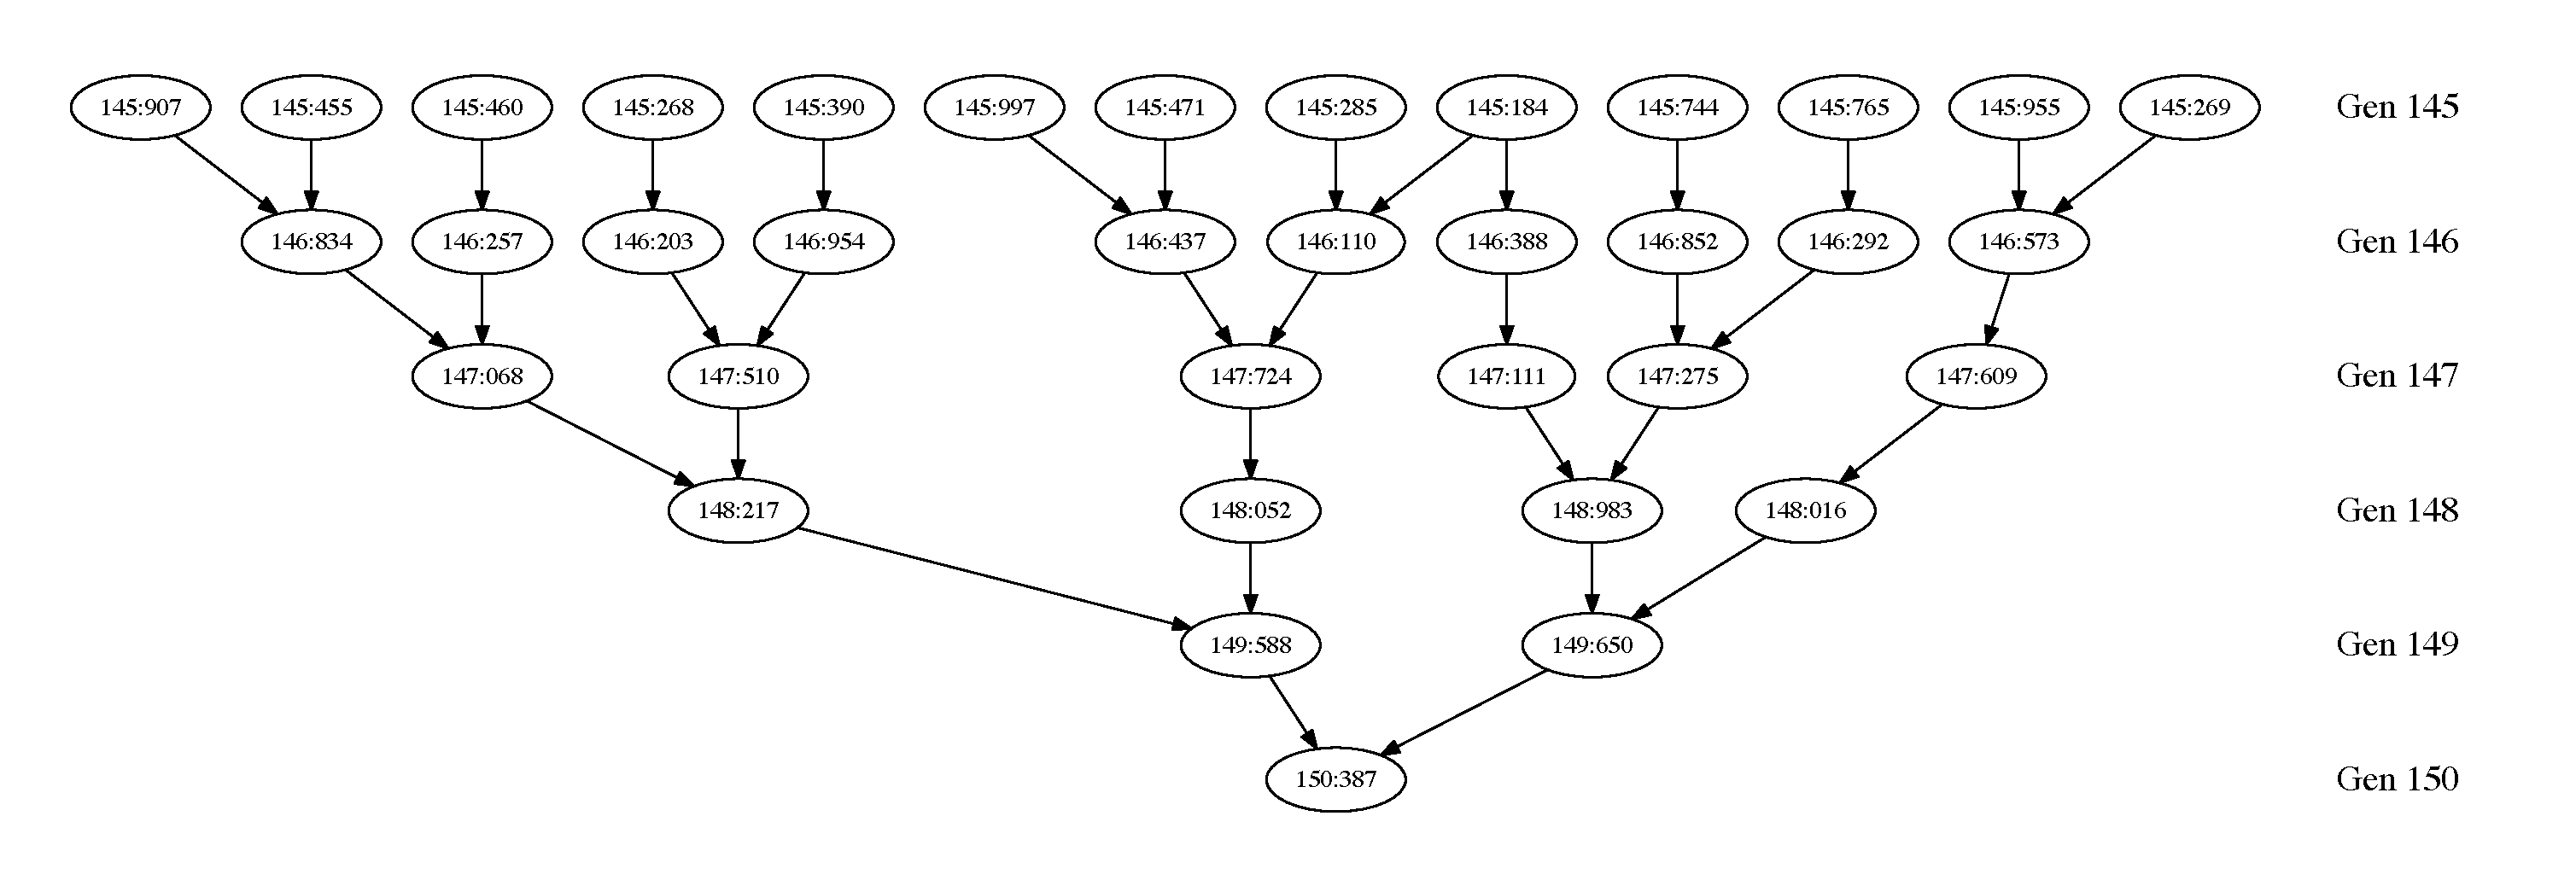
\includegraphics[width=\columnwidth]{figures/ancestors_of_winner_rswn_tourney_run74.pdf}
	\caption{Ancestry of the 45 ``winners'' from run 6 of lexicase, replace-space-with-newline. Nodes
		with diamonds instead of ellipses had an unusually large number of offspring. Shaded nodes
		had an unusual number of offspring that were ancestors of winners. The dashed lines highlight
		individuals that had an unusually large number of distinct ancestry paths down to a winner.
		See the text for more details}
	\label{fig:winnerAncestorsTourneyRun74}
\end{sidewaysfigure}

\section{Tournament Selection vs. Lexicase Selection}
\label{sec:1}

%logs/log30.txt
%logs/log41.txt
%logs/log50.txt
%logs/log52.txt
%logs/log60.txt
%logs/log62.txt
%logs/log64.txt
%logs/log68.txt
%logs/log6.txt
%logs/log74.txt
%logs/log82.txt
%logs/log94.txt
%logs/log96.txt

In addition to studying lexicase selection, we wanted to collect data from replace-space-with-new-line with tournament selection in order to compare lexicase versus tournament. As previously stated in section~\ref{meetLexicase}, lexicase  produced at least one individual with an error of zero in 55 of 100 runs while tournament selection only produced 13 of 100 successful runs. Of these 13 successful tournament runs, we selected one run to study based on the error diversity in the population over time that seemed to exhibit the similar error diversity trait as a majority of the other successful runs. Similarly, in selecting the lexicase run, we noticed that there were interesting dips in the amount of clusters over time and selected a lexicase run that emphasized that trait. 

An immediate difference that we noticed between the two runs was the number of individuals that solved the problem in the final generation. In lexicase, there were 45 different individuals that solved the problem while there was only a single individual in the tournament run that had an error of zero. 

Another major difference was the selection pressure of the style of selections. In lexicase selection, one parent can dominate the selection if it performs well for a majority of the test cases as we saw in section~\ref{sec:surprisingFecundity} where individual 86:261 was a parent for all but  approximately 70 individuals in the final generation. However, tournament selection never can have this level of selection pressure. Throughout the entire run, a single parent only produced 24 children at maximum. Comparing this to the lexicase selection there were over 40 parents that produced at least 100 children. This is an extreme difference in selection pressure between the two types of selections. 

Beside selection pressure, we noticed another crucial difference between the types of individuals selected for reproduction. With tournament selection, there is a biased towards individuals that have the lowest fitness. However, this is not the case in lexicase.  As long as an individual performs extremely well for many cases but not all, it is still possible to be selected for reproduction. In Table~ \ref{table:winnerFitnesses}, individual 85:086 has an error of 100,000. This late into the run, it would be very unlikely that tournament would select this individual to reproduce. In fact, we see this in the tournament run where there isn't a individual selected in the winning ancestry that has a total error of more than 132. Additionally, we noticed that the winning ancestry six generation back contained individuals with a total error of either 83 or 132. 


\section{Section Heading}
\label{sec:2}
% Always give a unique label
% and use \ref{<label>} for cross-references
% and \cite{<label>} for bibliographic references
Instead of simply listing headings of different levels we recommend to
let every heading be followed by at least a short passage of text.
Further on please use the \LaTeX\ automatism for all your
cross-references and citations.

Please note that the first line of text that follows a heading is not indented, whereas the first 
lines of all subsequent paragraphs are.

Use the standard \verb|equation| environment to typeset your equations, e.g.
%
\begin{equation}
a \times b = c\;,
\end{equation}
%
however, for multiline equations we recommend to use the \verb|eqnarray| environment.
\begin{eqnarray}
a \times b = c \nonumber\\
\vec{a} \cdot \vec{b}=\vec{c}
\label{eq:01}
\end{eqnarray}

\subsection{Subsection Heading}
\label{subsec:2}
Instead of simply listing headings of different levels we recommend to
let every heading be followed by at least a short passage of text.
Further on please use the \LaTeX\ automatism for all your
cross-references\index{cross-references} and citations\index{citations}
as has already been described in Sect.~\ref{sec:2}.

\begin{quotation}
Please do not use quotation marks when quoting texts! Simply use the \verb|quotation| environment -- it will automatically render Springer's preferred layout.
\end{quotation}


\subsubsection{Subsubsection Heading}
Instead of simply listing headings of different levels we recommend to
let every heading be followed by at least a short passage of text.
Further on please use the \LaTeX\ automatism for all your
cross-references and citations as has already been described in
Sect.~\ref{subsec:2}, see also Fig.~\ref{fig:1}\footnote{Footnotes are easily added with this simple command.}

Please note that the first line of text that follows a heading is not indented, whereas the first lines of all subsequent paragraphs are.

% For figures use
%
\begin{figure}[b] %[b] sets the image at the bottom of the page; t = top, b = bottom, h = here%
\sidecaption
% Use the relevant command for your figure-insertion program
% to insert the figure file.
% For example, with the graphicx style use
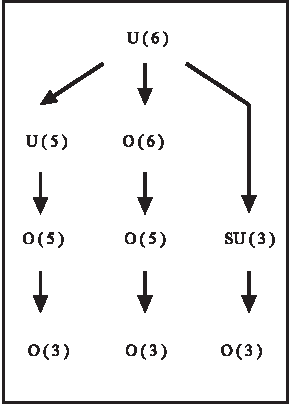
\includegraphics[scale=.65]{figure}
%
% If no graphics program available, insert a blank space i.e. use
%\picplace{5cm}{2cm} % Give the correct figure height and width in cm
%
\caption{If the width of the figure is less than 7.8 cm use the \texttt{sidecapion} command to flush the caption on the left side of the page. If the figure is positioned at the top of the page, align the sidecaption with the top of the figure -- to achieve this you simply need to use the optional argument \texttt{[t]} with the \texttt{sidecaption} command}
\label{fig:1}       % Give a unique label
\end{figure}


\paragraph{Paragraph Heading} %
Instead of simply listing headings of different levels we recommend to
let every heading be followed by at least a short passage of text.
Further on please use the \LaTeX\ automatism for all your
cross-references and citations as has already been described in
Sect.~\ref{sec:2}.

Please note that the first line of text that follows a heading is not indented, whereas the first lines of all subsequent paragraphs are.

For typesetting numbered lists we recommend to use the \verb|enumerate| environment -- it will automatically render Springer's preferred layout.

\begin{enumerate}
\item{Livelihood and survival mobility are oftentimes coutcomes of uneven socioeconomic development.}
\begin{enumerate}
\item{Livelihood and survival mobility are oftentimes coutcomes of uneven socioeconomic development.}
\item{Livelihood and survival mobility are oftentimes coutcomes of uneven socioeconomic development.}
\end{enumerate}
\item{Livelihood and survival mobility are oftentimes coutcomes of uneven socioeconomic development.}
\end{enumerate}


\subparagraph{Subparagraph Heading} In order to avoid simply listing headings of different levels we recommend to let every heading be followed by at least a short passage of text. Use the \LaTeX\ automatism for all your cross-references and citations as has already been described in Sect.~\ref{sec:2}, see also Fig.~\ref{fig:2}.

For unnumbered list we recommend to use the \verb|itemize| environment -- it will automatically render Springer's preferred layout.

\begin{itemize}
\item{Livelihood and survival mobility are oftentimes coutcomes of uneven socioeconomic development, cf. Table~\ref{tab:1}.}
\begin{itemize}
\item{Livelihood and survival mobility are oftentimes coutcomes of uneven socioeconomic development.}
\item{Livelihood and survival mobility are oftentimes coutcomes of uneven socioeconomic development.}
\end{itemize}
\item{Livelihood and survival mobility are oftentimes coutcomes of uneven socioeconomic development.}
\end{itemize}

\begin{figure}[t] %[t] sets the image at the top of the page; t = top, b = bottom, h = here%
\sidecaption[t]
% Use the relevant command for your figure-insertion program
% to insert the figure file.
% For example, with the option graphics use
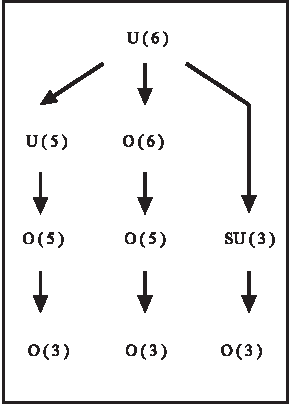
\includegraphics[scale=.65]{figure}
%
% If no graphics program available, insert a blank space i.e. use
%\picplace{5cm}{2cm} % Give the correct figure height and width in cm
%
%\caption{Please write your figure caption here}
\caption{If the width of the figure is less than 7.8 cm use the \texttt{sidecapion} command to flush the caption on the left side of the page. If the figure is positioned at the top of the page, align the sidecaption with the top of the figure -- to achieve this you simply need to use the optional argument \texttt{[t]} with the \texttt{sidecaption} command}
\label{fig:2}       % Give a unique label
\end{figure}

% Use the \index{} command to code your index words
% Make sure to inlcude the indexed word inside and outside of the brackets if you want the text to show up in your paragraph:
% e.g. This book is about \index{genetic programming}genetic programming. 
% If the text is not entered outside the brackets it will appear as: This book is about .
%
% For tables use
%
\begin{table}
\caption{Please write your table caption here}
\label{tab:1}       % Give a unique label
%
% Follow this input for your own table layout
%
\begin{tabular}{p{2cm}p{2.4cm}p{2cm}p{4.9cm}}
\hline\noalign{\smallskip}
Classes & Subclass & Length & Action Mechanism  \\
\noalign{\smallskip}\svhline\noalign{\smallskip}
Translation & mRNA$^a$  & 22 (19--25) & Translation repression, mRNA cleavage\\
Translation & mRNA cleavage & 21 & mRNA cleavage\\
Translation & mRNA  & 21--22 & mRNA cleavage\\
Translation & mRNA  & 24--26 & Histone and DNA Modification\\
\noalign{\smallskip}\hline\noalign{\smallskip}
\end{tabular}
$^a$ Table foot note (with superscript)
\end{table}
%
\section{Section Heading}
\label{sec:3}
% Always give a unique label
% and use \ref{<label>} for cross-references
% and \cite{<label>} for bibliographic references
Instead of simply listing headings of different levels we recommend to
let every heading be followed by at least a short passage of text.
Further on please use the \LaTeX\ automatism for all your
cross-references and citations as has already been described in
Sect.~\ref{sec:2}.

Please note that the first line of text that follows a heading is not indented, whereas the first lines of all subsequent paragraphs are.

If you want to list definitions or the like we recommend to use the Springer-enhanced \verb|description| environment -- it will automatically render Springer's preferred layout.

\begin{description}[Type 1]
\item[Type 1]{That addresses central themes pertainng to migration, health, and disease. In Sect.~\ref{sec:1}, Wilson discusses the role of human migration in infectious disease distributions and patterns.}
\item[Type 2]{That addresses central themes pertainng to migration, health, and disease. In Sect.~\ref{subsec:2}, Wilson discusses the role of human migration in infectious disease distributions and patterns.}
\end{description}

\subsection{Subsection Heading} %
In order to avoid simply listing headings of different levels we recommend to let every heading be followed by at least a short passage of text. Use the \LaTeX\ automatism for all your cross-references and citations citations as has already been described in Sect.~\ref{sec:2}.

Please note that the first line of text that follows a heading is not indented, whereas the first lines of all subsequent paragraphs are.

\begin{svgraybox}
If you want to emphasize complete paragraphs of texts we recommend to use the newly defined Springer class option \verb|graybox| and the newly defined environment \verb|svgraybox|. This will produce a 15 percent screened box 'behind' your text.

If you want to emphasize complete paragraphs of texts we recommend to use the newly defined Springer class option and environment \verb|svgraybox|. This will produce a 15 percent screened box 'behind' your text.
\end{svgraybox}


\subsubsection{Subsubsection Heading}
Instead of simply listing headings of different levels we recommend to
let every heading be followed by at least a short passage of text.
Further on please use the \LaTeX\ automatism for all your
cross-references and citations as has already been described in
Sect.~\ref{sec:2}.

Please note that the first line of text that follows a heading is not indented, whereas the first lines of all subsequent paragraphs are.

\begin{theorem}
Theorem text goes here.
\end{theorem}
%
% or
%
\begin{definition}
Definition text goes here.
\end{definition}

\begin{proof}
%\smartqed
Proof text goes here.
\qed
\end{proof}

\paragraph{Paragraph Heading} %
Instead of simply listing headings of different levels we recommend to
let every heading be followed by at least a short passage of text.
Further on please use the \LaTeX\ automatism for all your
cross-references and citations as has already been described in
Sect.~\ref{sec:2}.

Note that the first line of text that follows a heading is not indented, whereas the first lines of all subsequent paragraphs are.
%
% For built-in environments use
%
\begin{theorem}
Theorem text goes here.
\end{theorem}
%
\begin{definition}
Definition text goes here.
\end{definition}
%
\begin{proof}
\smartqed
Proof text goes here.
\qed
\end{proof}
%
\begin{acknowledgement}
If you want to include acknowledgments of assistance and the like at the end of an individual chapter please use the \verb|acknowledgement| environment -- it will automatically render Springer's preferred layout.
\end{acknowledgement}

\bibliographystyle{spbasic}
\bibliography{gp-bibliography,chapter}
